\subsection{拓扑除环上的一致结构}

若 K 是拓扑除环，就必须区分：1) K 的加法群的一致结构，它定义在 K 上，称为 K 的加法一致结构；与 2) 乘法群 \(\mathbf{K}^*\) 的左一致结构与右一致结构，它们定义在 \(\mathbf{K}^*\) 上，并（按用语之便）称为 K 的乘法一致结构。

由 K 的加法一致结构在 \(K^{*}\) 上诱导的一致结构一般不同于 K 的乘法一致结构（见习题 17）。

由命题 6，豪斯多夫拓扑除环 K 可以看作完备豪斯多夫环 \(\hat{K}\) 的一个稠密子环。为使 \(\hat{K}\) 是拓扑除环，必须映射 \(x \to x^{-1}\) 可由连续性延拓到 \((\hat{\mathbf{K}})^{*}\) 上；而这个必要条件也是充分的，因为这时函数 \(xx^{-1}, x^{-1}x\) 与 \(1\) 由恒等延拓原理在 \((\hat{\mathbf{K}})^{*}\) 上相等，因此延拓后的函数的值是 \(x\) 的逆，这里 \(x \neq 0\) 取遍 \(\hat{\mathbf{K}}\)。换句话说（参见第二章，§ 3，第 6 节，命题 11）：

命题 7. 完备化 \(\hat{\mathbf{K}}\)——豪斯多夫拓扑除环 \(\mathbf{K}\) 的完备化——是拓扑除环，当且仅当在映射 \(x \to x^{-1}\) 下，每个不以 0 为聚点的（关于加法结构的）Cauchy 滤子的像，都是（关于加法结构的）Cauchy 滤子。

\pandocbounded{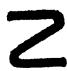
\includegraphics[keepaspectratio]{images/part002_56877e98.jpg}}

存在这样的拓扑除环，其中这一条件不满足，且其中环 \(\hat{\mathbf{K}}\) 有零因子（见习题 26）。此外，即使完备化 \(\hat{\mathbf{K}}\) 是拓扑除环，也没有先验的理由认为 \(\hat{\mathbf{K}}\) 的乘法一致结构是完备空间的结构。然而，对于除环 \(\mathbf{K}\)——只要 \(\hat{\mathbf{K}}\) 局部紧（见第一章，§ 9，第 7 节，命题 13，及第三章，§ 3，第 3 节，命题 4）——以及对于拓扑域，情形就是如此；对后者，我们有下列命题：

命题 8. 若拓扑域 K 的加法一致结构是完备豪斯多夫空间的结构，则 \(K^{*}\) 上的乘法一致结构是完备空间的结构。

我们将证明，若 \(\mathfrak{F}\) 是 \(\mathbf{K}^*\) 上关于乘法一致结构的 Cauchy 滤子，则 \(\mathfrak{F}\) 是 \(\mathbf{K}\) 上关于加法一致结构的 Cauchy 滤子，且不收敛于 \(o\)；这样就证得了结果。设 \(\mathbf{U}\) 是 \(o\) 在 \(\mathbf{K}\) 中的一个任意邻域，设 \(\mathbf{V}\) 是 \(o\) 的闭邻域，使得 \(\mathbf{V} \subset \mathbf{U}\)、\(\mathbf{VV} \subset \mathbf{U}\){[}公理 \((\mathrm{AV}_{\mathrm{II}})]\) 且 \(-1 \notin V\)；则按假设存在集合 \(\mathbf{A} \in \mathfrak{F}\)，使得对所有 \(x \in \mathbf{A}\) 与 \(y \in \mathbf{A}\)，有 \(x^{-1}y \in 1 + V\)。取 \(a \in \mathbf{A}\)，则 \(\mathbf{A} \subset a + aV\)，而 \(a + aV\) 是不含 \(o\) 的闭集；因此 \(o\) 不在 \(\mathbf{A}\) 的闭包中，从而不是 \(\mathfrak{F}\) 的聚点。设 \(\mathbf{W}\) 是 \(o\) 的邻域，使得 \(aW \subset V\){[}公理 \((\mathrm{AV}_{\mathrm{I}})]\)；则按假设存在集合 \(\mathbf{B} \in \mathfrak{F}\)，使得 \(\mathbf{B} \subset \mathbf{A}\)，且对所有 \(x \in B\) 与 \(y \in B\)，有 \(x^{-1}y \in 1 + W\)；于是 \(y - x \in xW \subset AW \subset aW + aVW\)；但 \(\mathbf{K}\) 交换，因此 \(aVW = aWV \subset VV \subset U\)；从而 \(y - x \in U + U\)，命题得证。

同样的证明表明，命题 8 可以推广到如下的情形：关于 K 的两个乘法一致结构之一的每个 Cauchy 滤子，也是关于另一个乘法一致结构的 Cauchy 滤子。

